\scanpage{8}
\mspage{6}
\margin{\figure{\begin{tikzpicture}\draw (0,0)--(.5,-.65);\end{tikzpicture}}}

\figure{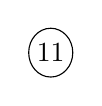
\begin{tikzpicture}[baseline=(t.base)]\node (t) {11};\draw (0,0) ellipse (0.28 and 0.31);\end{tikzpicture}}
pg101\quad $\ell-6$.\quad Dire où on trouve que Néron commute à $S\mapsto\widehat S$.

pg103\quad Le renvoi au courage du lecteur est désagréable --
\margin{\figure{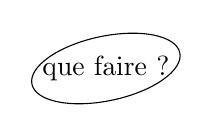
\begin{tikzpicture}[baseline=(t.base)]\node (t) {que faire ?};\draw[rotate=12] (0,0) ellipse (0.96 and 0.41);\end{tikzpicture}}}

Si j'ai bien compris, tu affirme que prolonger une biextension à $A\times A'$ est ``la $\hat{\mathrm m}$ chose'' que de la prolonger aux ${}_{\ell^\infty}A\times{}_{\ell^\infty}A'$.

\margin{7}
